\section{The LHCb detector}
\label{sec:detector}

The large hadron collider (LHC) located at CERN near Geneva is the largest particle accelerator to date.
Opposing proton beams are collided at four different interaction points with center of mass energies up to \qty{13}{\tera\electronvolt}.
Every interaction point houses one experiment, with each of them having a detector that is optimized for a different physics purpose.
The four experiments are called ALICE, ATLAS, CMS and LHCb. The data used in this analysis is recorded at the LHCb detector.
This detector is optimized for the study of $b$ physics and measurements of CP violation parameters, which is exactly the type of physics
present in the $B$ meson decays that are analysed in this lab course.

The LHCb detector is a single-arm forward spectrometer, this particular design was chosen because the particles studied at LHCb are mainly produced
with a strong boost in the forward direction. The polar anglular coverage reaches from $15$ to $\qty{300}{\milli\radian}$ \cite{LHCbMVA}.
A schematic view of the LHCb detector can be seen in \autoref{fig:lhcb} at the status during the first data-taking period.
Here, the $z$-axis is along the beam direction, the negative $z$-region is referred to as upstream, while the positive $z$-region is called downstream.

\begin{figure}[H]
	\centering
	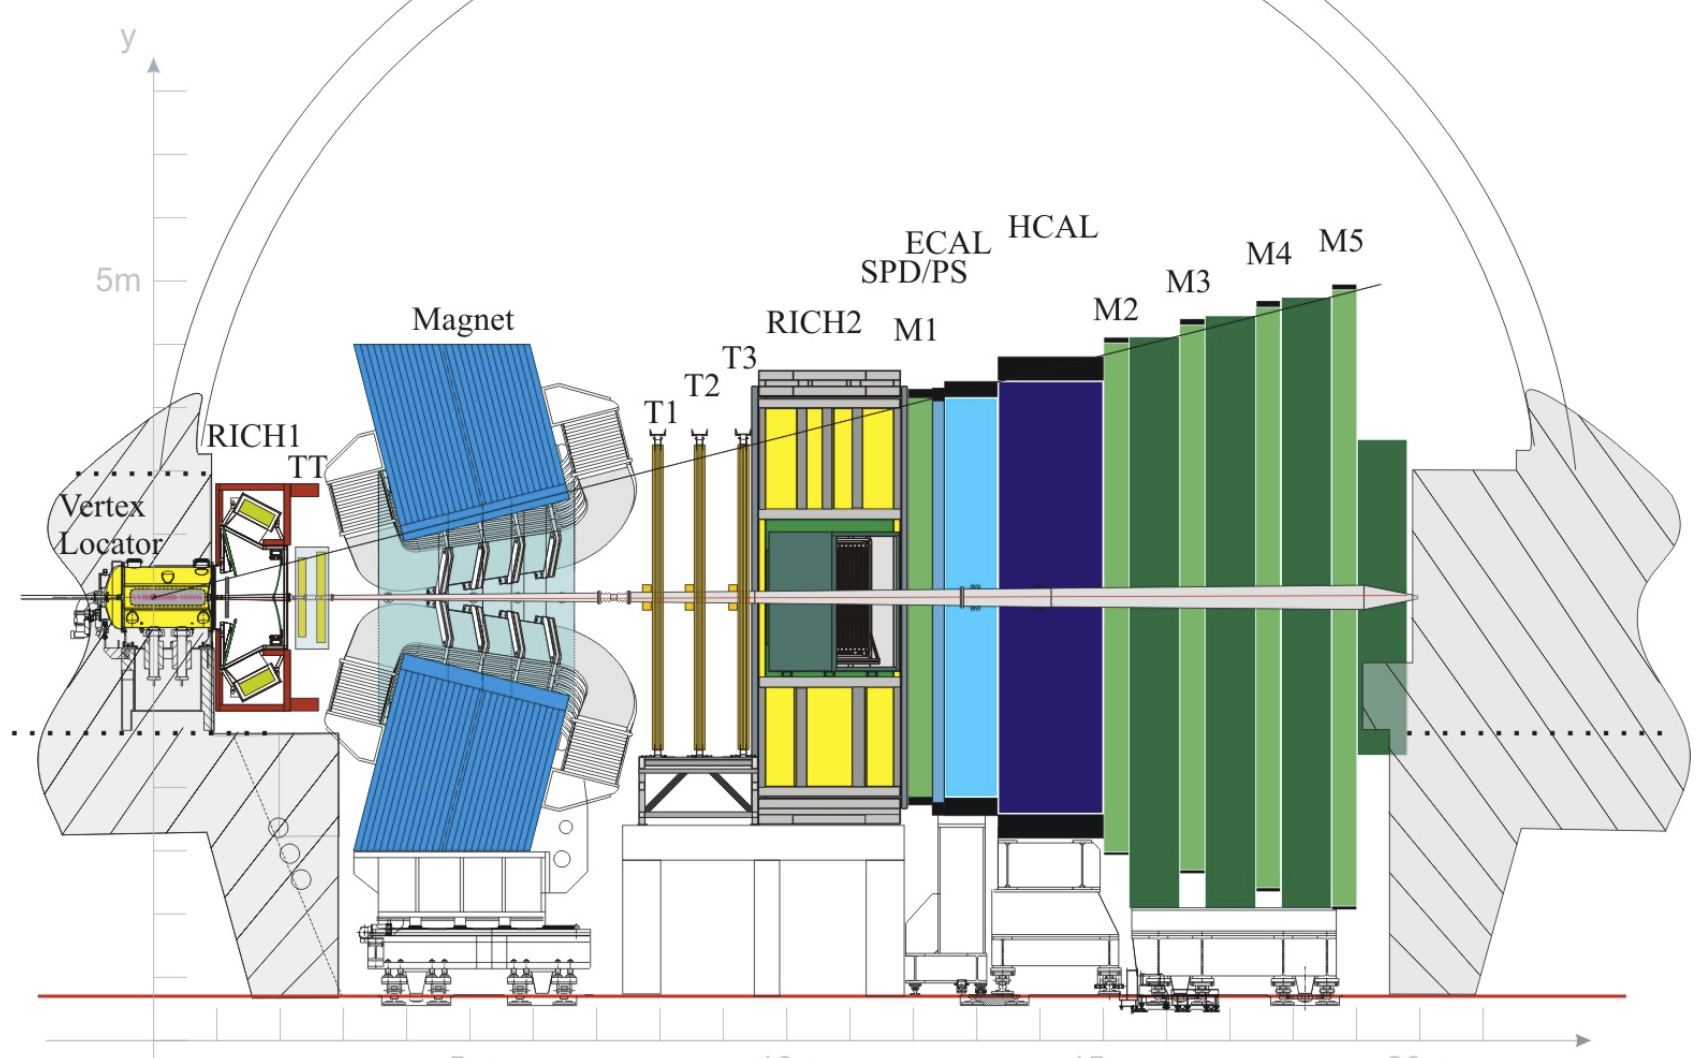
\includegraphics[width=0.7\linewidth]{content/pictures/lhcb.png}
	\caption{Cross-section of the LHCb detector, the following components are shown from left to right: The vertex locator (VELO),
		the Cherenkov detectors (RICH1,RICH2), the tracking system (TT and T1,T2,T3) including the magnet,
		the calorimeters (ECAL, HCAL) and the muon chambers (M1-M5).}
	\label{fig:lhcb}
\end{figure}

The first component of the detector is the vertex locator (VELO), it is located directly at the interaction point. The VELO consits of multiple
silicon strip detectors, meant to reconstruct the position of the proton-proton interaction, the primary vertex, and the decay location of the $b$ hadron (secondary vertex).
The $B$ mesons typically have a flight path length of a few $\si{\milli\meter}$ to $\si{\centi\meter}$ and thus decay directly inside the VELO.
The Ring Imaging Cherenkov (RICH) detectors 1 and 2 are used to calculate the velocity of transversing particles. This is archieved by measuring the diameter of light cones emitted by these 
particles due to the Cherenkov effect. \\
To obtain information about the particles momentum and charge, they are deflected by a dipole magnet with an integrated field strength of about \qty{4}{\tesla\meter}. Charged particles
will then travel on a curved track. The tracking stations TT and T1-3 consit of large-area, four-layer silicon strip detectors as well as drift tubes. They measure the
curved particle tracks and thus their radius can be determined. This allows it to calculate the momentum of the particle, while its charge is given by the direction of the particles deflection
in the magnet. Combining the information about particle momentum, velocity and charge allows for particle identification (PID).
Further downstream lies the calorimeter system, it is divided into the electromagnetic (ECAL) and hadronic (HCAL) calorimeters.
The main purpose of the calorimeters is the measurement of the energy deposited by photons and electrons in the ECAL and hadrons in the HCAL, respectively.
Additionally the calorimeters also contribute to PID. The last main components are the five muon stations located at the end of the detector. Here, muons that traverse all other
detector parts without much interaction can be measured. \\
While the proton proton collisions occur at a rate of \qty{11}{\mega\hertz}, event storage is only possible with a rate of \qty{3}{\kilo\hertz} \cite{LHCbMVA}. To reduce the
number of events, only physically interesting events are selected via a trigger system consisting of a hardware and software implementation.

\section{Analysis strategy}
For this analysis three types of samples are provided. Two simulation samples of the \signal \ decay used as a signal proxy as well as the so-called control channel, a kinematically similar decay channel $B \to \psi(2S)K_S$ and the actual data sample. This data sample contains candidates from both the signal and control channel as well as the background candidates. For the later training of the classifier the so-called upper sideband (candidates with a invariant mass higher outside the signal region) of the data sample is used as a proxy for background.\\

As the distributions in the control and signal channel differ from those in the actual data sample it is necessary to align these. This so called \textit{kinematic reweighting} has already been performed. As these generated weights align only some of the distributions in the samples it is important to find those deviating to much. These features are determined using \textit{largest distance between the cumulative probability distributions} $F^i$
\begin{equation*}
	\underset{n}{\mathrm{sup}}\left|F^1_n - F^2_n\right|,
\end{equation*}
where $F^i$ is determined form histogramming the different features.